\section*{Functionel Description Report}
\tableofcontents
\newpage

\section{Abstract}
\textbf{\textit{This report will outline the functionality and theory of our project for Cybertechnology in course 34229}}. The projects fundamental goal is to explore and examine 802.11. The focus will be on exploring how management frames can be exploited for malicious use and how this can be mitigated. The main focus is on how an Evil Twin Attack can be performed from start to end. Further a side focus will be on the different authentication protocols in regards to password cracking. Thus in this project it has been possible to scan and identify the local wireless networks in the area, hereby giving the ability to deauthenticate clients and emulating a rogue AP for the clients to connect to, hence achieving a man-in-the-middle like state. Lastly it has been possible to crack/obtain a WEP password via sniffing.





\section{Introduction}

Security in wireless networks has become increasingly important do to the rapidly expanding use and need for internet access. However, even with the many security measures in place for wireless networks, there are still vulnerabilities to attacks on said networks. One such attack is the deauthentication attack. Wherein a user will be rejected access to the network he/she is attempting to create a connection to.

This project will, explore the theory and practical applications of deauthentication attacks on networks. Furthermore we will investigate the cracking of passwords used in the encryption of wireless network traffic using WEP. To achieve this, we will need to gain full knowledge of the wireless local area network. Therefore another goal for the project is to create a table of available wifi's, along with information on clients connected, signal strength and much more.

Through this project, we aim to highlight the vulnerabilities of wireless networks and demonstrate the importance of securing them. It is important to note that this project is for educational purposes only and should not be used for malicious activities. Overall, this project will provide a comprehensive understanding of the vulnerabilities of wireless networks and the importance of implementing strong security measures.

\iffalse
2 De tre søjler
2.1 Mapping af netværk
    Det skal være muligt at sige alt om sit WLAN:
    • hvor mange WiFi er der (herunder alle AP’s p ̊a hvert WiFi)
    • Hvor mangle klienter findes der (svært ved randomization af MAC (fint teori-afsnit))
    • Hvilken klienter er logget ind p ̊a hvilken netværk
    • Er MAC-adresse en klient eller AP (from-ds/to-ds)
    • Hvor langt/tæt p ̊a er de
    • Hvilke kanaler er meget i brug
    • Evt. s ̊arbarhedsscanning
2.2 Deauth (Evil Twin)
    Det skal være muligt at DoS:
    • Klient
    • AP
    • Kanal
    Ligeledes skal der udforskes, hvorvidt disse DoS kan mitigeres og/eller opdages. god
    at udfolde - henrik Hvis tiden er til det, vil det ogs ̊a være spændende at udnytte deauth til at
    tvinge klienter hen p ̊a et rogue AP (man-in-the-middle).
2.3 Password cracking og WEP/WPA2
    Her opsætter man at man kan bryde den lette password algoritme WEP og ogs ̊a at vise hvordan
    WPA2 forbedrer p ̊a sikkerhden i forhold til WEP. Den bliver meget teoretisk og der skal kommes
    ind p ̊a hvordan WEP og WPA fungerer. Man kan lave nogle matematiske udregninger der viser
    hvor langt tid det gennemsnitligt vil tage at bryde forskellige passwords i WEP og WPA2, som
    tydeligt viser at WPA2 er bedre. Der skal laves kode som bryder pakker med WEP sikkerhed,
    som vi nok selv har lavet, da WEP ikke længere bruges.
\fi




\section{Functionality}
Our project is made up of these functionalities:
\begin{enumerate}
    \item Scan local networks (Maybe even identify)
    \item Become an AP
    \item Deauthentication attacks
    \item Password cracking
\end{enumerate}

 
These functionalities aim to be the core of the product that will be created. The first functionality, Scanning for local networks, is the most important one as that is the basis of all other functionalities. 
Becoming an AP is the function that allows the product to allow Wi-Fi devices to connect to the product. It acts as a central transmitter and receiver of the wireless radio signals. 

A deauthentication attack is a type of denial-of-service attack that targets communication between a user and a Wi-Fi wireless access point. It exploits a feature of IEEE 802.11 wireless networks that allows devices to disconnect from a network by sending deauthentication frames.

A deauthentication frame is a message that tells a device to stop using the network. It can be sent by either the access point or the device itself. Normally, it is used for legitimate purposes, such as ending a connection or switching to another network.

However, an attacker can also send deauthentication frames to any device associated with an access point, using a tool such as Aircrack-ng3 or in our case Scapy. This causes the device to lose its connection and try to reconnect, which consumes bandwidth and resources. If done repeatedly or to multiple devices, this can disrupt or disable the network entirely.

The last point is password cracking. The product should be able to crack basic passwords in the WEP algorithm as that is one of the most basic security algorithms. It is and outdated and insecure algorithm and the product can use some of the multitude of tools available to crack it, like Aircrack-ng's PTW and FMS or WEPcrack. Alternatively we can create our own algorithm for cracking WEP if time permits.

We are going to write in python using Scapy to implement the functions \cite{scapy}. We are also using Debian Linux to allow monitor mode on the wireless network cards. Hopefully we can use a raspberry pi later in the project when all the code has been written and is easily able to be placed onto the raspberry pi. 
If we are not able to use a raspberry pi the product will use a Realtek DWA 131-E1 dongle that creates a wlan adapter and allows monitor mode. This has the consequence that linux is required and that everything runs through a python program on a computer.
The positive side of using linux is that we can implement the program on many types of systems as we use a VM to create the product and makes conversion to a raspberry pi easier. The negative side is that we have to use a VM which can create problems with drivers and performance. 

\section{Blocks and sub-blocks}

This project will be built on 3 main blocks, "Mapping of networks", "Deauthentication" and "Password cracking". In in these blocks will be sub-blocks containing functionality for the specific block. 

\subsection{Mapping of networks}
This block takes the physical data being sent in the wireless space, and transforms it into information that the other blocks need and use. It contains a table that holds the information as sub-blocks, for instance wifi' in the local area, as well as the clients on said wifi. Or the signal strength of the wifi and which channels are used the most.

\subsection{Deauthentication}
This block is all about deauthentication, where we deny clients usage of certain WiFi's, AP's or all wireless internet usage. So the natural sub-blocks in this block are: 
\begin{itemize}
    \item Client
    \item AP
    \item Channel
\end{itemize}

The induvidual sub-blocks each then are a class that do each thing. 

\subsection{Password cracking and WEP/WPA2}
This block is mainly about WEP and how to crack it, but is also about generally how to secure a WiFi or AP with passwords and how long it takes to crack WEP vs WPA2. 



\section{Theory}
The main theory behind this project is the 802.11 standard \cite{IEEE802.11}.
The 802.11 standard, is a set of wireless network protocols developed by the Institute of Electrical and Electronics Engineers (IEEE). The first version of the standard, 802.11, was released in 1997, and since then, several revisions and amendments have been made to improve the technology and increase its capabilities.

The 802.11 standard uses radio waves to transmit data between devices within a local area network (LAN) without the need for cables or wires. This makes it a popular choice for connecting devices to the internet, especially in homes, offices, and public places such as cafes, airports, and hotels.

The original 802.11 standard operated in the 2.4 GHz frequency band. However, subsequent versions, including 802.11b, 802.11a, 802.11g, and 802.11n, increased the data rate and expanded the frequency band to include 5 GHz.

802.11b was the first widely adopted WiFi standard, released in 1999, and provided a maximum data rate of 11 Mbps. It operates in the 2.4 GHz frequency band and is backward compatible with the original 802.11 standard.

802.11a, released in 1999, operates in the 5 GHz frequency band and provides a maximum data rate of 54 Mbps. However, due to its shorter range compared to 802.11b, it was not as widely adopted.

802.11g, released in 2003, operates in the 2.4 GHz frequency band and provides a maximum data rate of 54 Mbps. It is backward compatible with 802.11b and became the dominant WiFi standard for several years due to its high data rate and compatibility with older devices.

802.11n, released in 2009, improved the data rate further, with a maximum of 600 Mbps. It uses both the 2.4 GHz and 5 GHz frequency bands and introduced multiple input multiple output (MIMO) technology, which allows for multiple antennas to transmit and receive data simultaneously. This improves the signal strength and range of the network.

Throughout the project, programming will be done mainly in python, using the library Scapy for sniffing, analysis and transmission packets. Scapy is a program written in Python, that gives the ability to construct, decrypt, send, capture packets and much more\cite{IEEE_Scapy}. Scapy gives us tools for analyzing 802.11 frames, thus providing the information contained in 801.11 frames. Packets in Scapy are created as objects with layers built on top of each other to define the type of the packet.





\begin{figure}[!htbp]
    \centering
    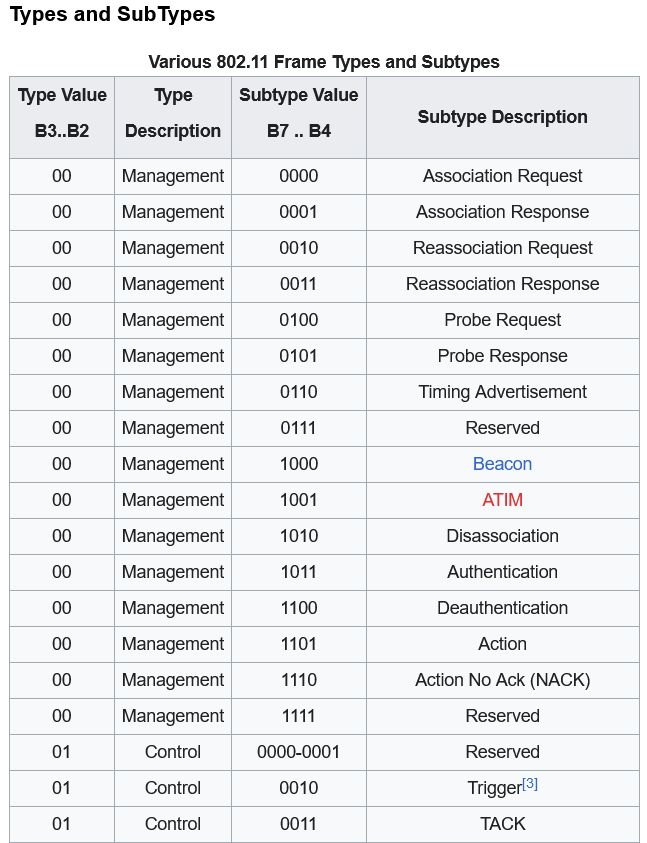
\includegraphics[width=0.6\textwidth]{Latex-Files/Billeder/WIFI_Types.png}
    \caption{WiFi typer og subtyper}
    \label{Wifi Types}
\end{figure}

In 802.11 there are 3 frame types: Management frames, control frames and data frames \cite{Amit802.11frames, DefinitiveGast}. Figure \ref{Wifi Types} shows some of the types and subtypes of different frames. Our focus is on management frames.  Management frames are used by AP's to join and leave the basic service set. They are needed because it is much harder to connect to a specific wireless network rather than a wired network as that is almost automatic when a wire is connected. A wireless network needs to associate a client with radio waves from a certain sender and ignore others. For clients to know which networks are around them they need to know data about them, this is done via 2 ways of scanning: Active scanning and passive scanning. In passive scanning the client scans every channel passively and listens for beacon frames from AP's, this has the consequence that clients can miss a beacon frame from an AP, since it has to go through every available channel. A beacon frame gives basic information about the AP and are sent continuously by every AP. In active scanning a client sends out probe requests on the channels and listens for probe responses from all the AP's that answer, this has the consequence that a client almost certainly gets information about every single AP in the area. The probe responses gives the client the SSID and capabilities of the AP's. 

Wireless networking also needs security while sending packets, some of this security being authentication and confidentiality. To ensure confidentiality data frames are encrypted with some sort of security standard. The oldest widespread type being Wired Equivalent Privacy (WEP). It had major security flaws that allows hackers to bypass the algorithm and read the data being sent\cite{WEP1}. Therefore was Wi-Fi Protected Access (WPA) developed in 2003. 

WEP uses a secret key to encrypt packets between client and AP\cite{WEP2}. The problem with it is that WEP uses the RC4 encryption algorithm, which is known as a stream cipher. A stream cipher operates by making a short key into an infinite random key-stream. The client uses XOR on the key-stream with the plain data to produce the encrypted data. The AP has a copy of the same used key, and uses it to generate identical an key-stream. The AP then uses XOR on the key-stream with the encrypted data to get the exact same plain data back. This type of encryption is easy to misuse as by flipping a single bit in the encrypted data, the plain data will also have a corresponding single bit flipped. Also the XOR can be found via statistical analysis of key-streams to thereby recover the plain data.

WEP has incorporated defenses against these 2 types of attacks, but they are implemented poorly. The defense against flipping bits are integrity checks in the packet implemented as a CRC-32 checksum. Sadly it is linear which means that it is possible to find the difference between 2 CRC's because the bits that are flipped in the encrypted data is deterministic and therefore an attacker can adjust the checksum and then it is believed that the integrity of the packet is kept, when in reality it isn't.

The defense against the statistical attack is an initialization vector to decrease the chance of reuse of key-streams. The vector is only a 24 bit field and that guarantees the reuse of key-streams. Because of this the attacker can easily pick up enough data to perform statistical analysis of packets using the same key-stream and then recover the plain data.

WPA2 was a development of the intermediate measure WPA, as a security update to fix many of WEP's problems \cite{WPA2_1}. It was released in 2004 in the 802.11i amendment to the original 802.11. WPA2 uses the AES security algorithm which rids the network of the previously mentioned security vulnerabilities. For a product to be WiFi certified it requires the usage of WPA2 \cite{WPA2_2}. New security vulnerabilities have since been found in WPA2 and WPA3 has been created to solve some of those and is planned to be implemented widepsread soon.

The authentication of clients and AP's can be exploited by deauthentication attacks. A deauthentication attack is a type of wireless network attack that involves sending forged deauthentication packets to a target client or AP. The theory behind this attack is based on the 802.11 standard, which allows clients to disconnect from an AP using a deauthentication packet.

When a client device is connected to a WiFi network, it sends periodic beacon packets to the access point to maintain the connection. In a deauthentication attack, an attacker sends a series of forged deauthentication packets to the target client or access point, pretending to be the legitimate access point or client. This causes the target to disconnect from the network and require reauthentication, disrupting the communication between the client and the access point.




\section{Conclusion}

We have investigated network traffic via mapping a local WiFi network using Python and the tool scapy to show all AP's connected and sending beacon frames and the clients connected to these networks. We also did deauthentication attacks to disconnect one or more clients from using wireless networking. By doing this we got advanced knowledge about different types of frames and subframes in the 802.11 standard. We also investigated security in the 802.11 standard, both WEP and WPA2, the 2 most common security algorithms for ensuring the security and integrity of packets and data-streams. 

\newpage
\section{Time Plan}
\begin{figure}[!htbp]
    \centering
    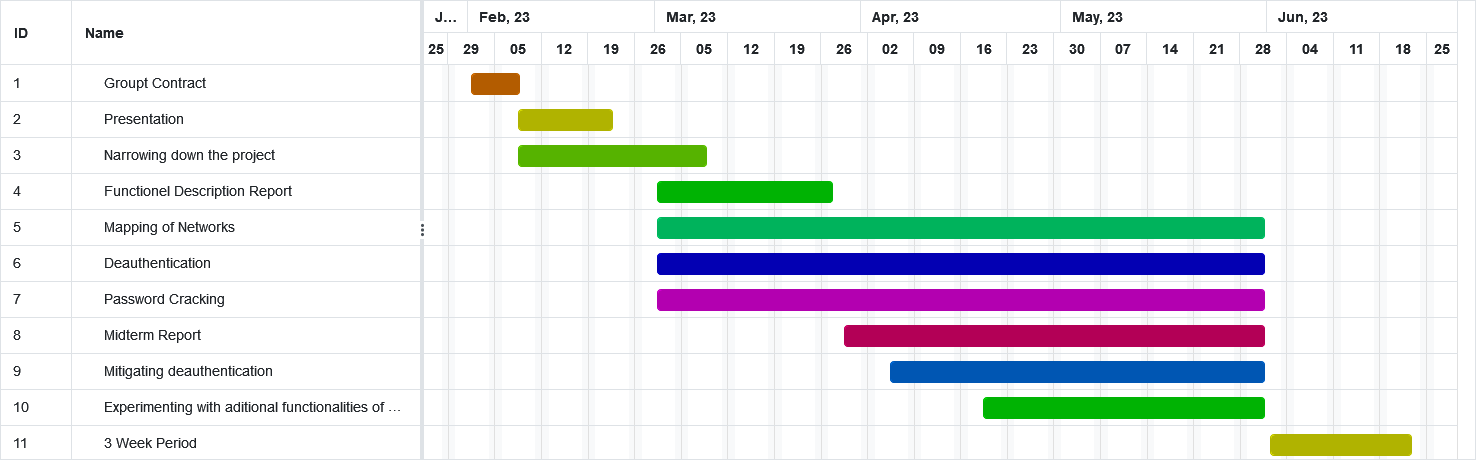
\includegraphics[width=1\textwidth]{Latex-Files/Billeder/Timeplan.png}
    \caption{Timeplan}
\end{figure}
